\chapter{Пример работы программы}

На рисунках~\ref{fig:1-seq}~---~\ref{fig:2-seq} показан пример работы программы в последовательном режиме. Программа последовательно обрабатывает три страницы сайта \url{gastronom.ru}, сохраняя данные рецепта с каждой страницы в отдельные файлы в формате $JSON$, которые размещаются в директории $recipes\_data$. Пример содержимого одного из таких $JSON$-файлов представлен на рисунке~\ref{fig:file}.

\begin{figure}[h]
	\centering
	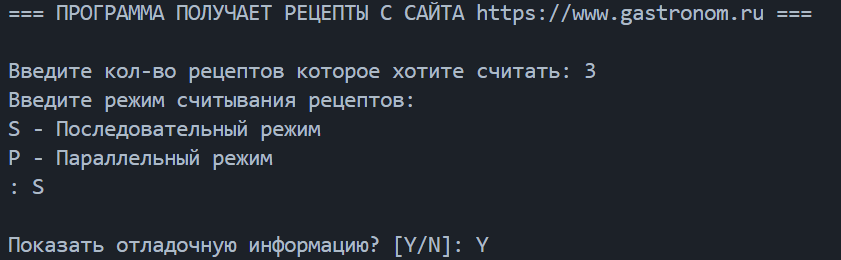
\includegraphics[width=0.8\textwidth]{images/examples/sin.png}
	\caption{Ввод данных в интерфейс приложения}
	\label{fig:1-seq}
\end{figure}
\begin{figure}[h]
	\centering
	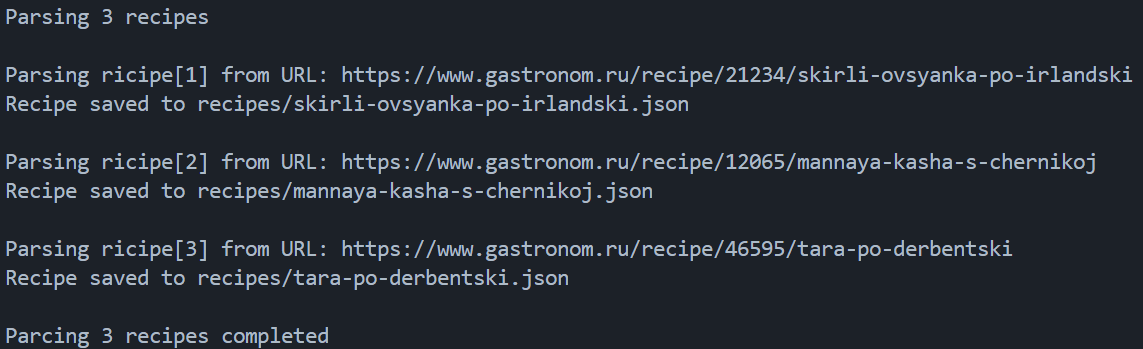
\includegraphics[width=0.8\textwidth]{images/examples/sout.png}
	\caption{Сообщения о ходе выполнения парсинга}
	\label{fig:2-seq}
\end{figure}


На рисунках~\ref{fig:1-paral}~---~\ref{fig:2-paral} представлен пример работы программы в параллельном режиме. В данном случае программа создает для обработки страниц заданное  количество потоков. После создания всех потоков и выдачи им задач главный поток блокируется на время парсинга всех страниц. Потоки сохраняют данные о рецепте в отдельные $JSON$-файлы, которые помещаются в директорию $recipes\_data$.

\begin{figure}[h]
	\centering
	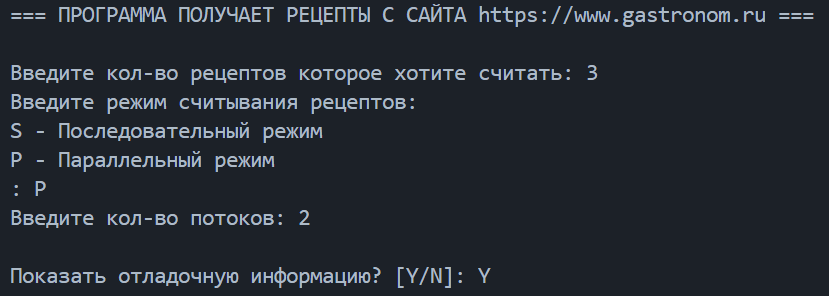
\includegraphics[width=0.8\textwidth]{images/examples/pin.png}
	\caption{Ввод данных в интерфейс приложения}
	\label{fig:1-paral}
\end{figure}
\begin{figure}[h]
	\centering
	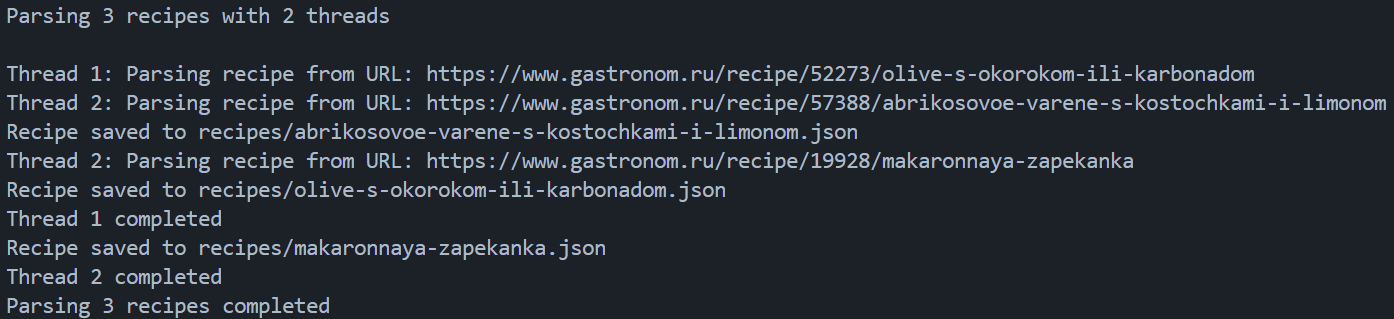
\includegraphics[width=0.8\textwidth]{images/examples/pout.png}
	\caption{Сообщения о ходе выполнения парсинга}
	\label{fig:2-paral}
\end{figure}

\begin{figure}[h]
	\centering
	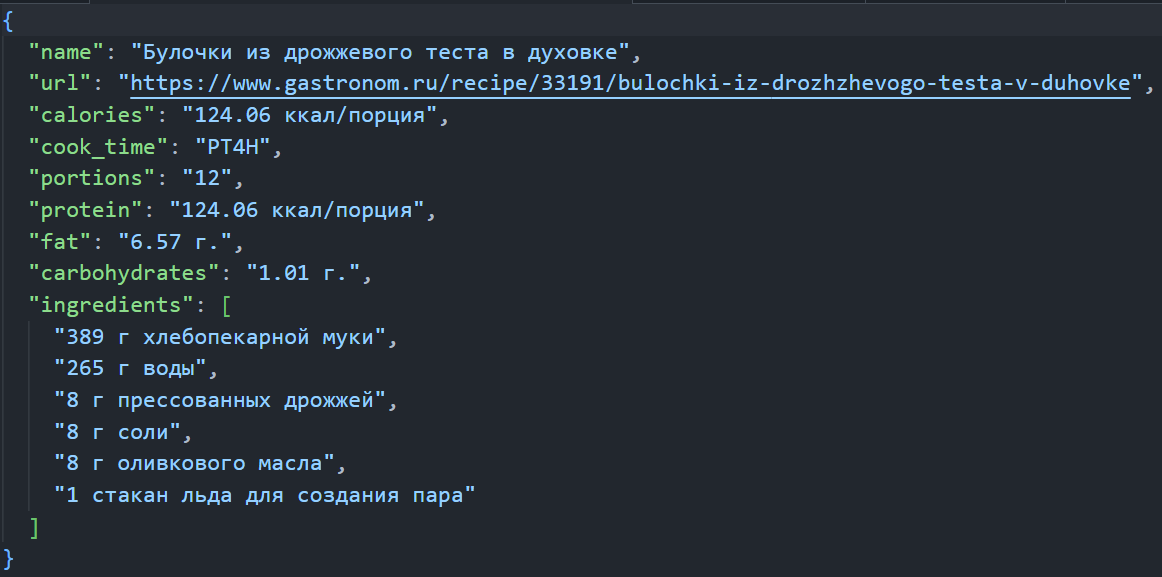
\includegraphics[width=0.8\textwidth]{images/examples/file.png}
	\caption{Содержимое выходного файла}
	\label{fig:file}
\end{figure}